\documentclass[9pt,a4paper,twocolumn]{article}
\usepackage[margin=0.9in]{geometry}
\usepackage{hyperref}
\usepackage[final]{pdfpages}
\usepackage{subcaption}
\usepackage{cite}
\usepackage[acronym]{glossaries}

 \setlength{\columnsep}{0.25in}

\makeglossaries

\newacronym{scc}{SCC}{Strongly Connected Components}

\title{An Analysis of the Portuguese Section of Wikipedia}

\author{Daniel Ramos \\ 81620 \and Miguel Tavares \\ 83528 \and Ricardo Brancas  \\ 83557}

\begin{document}
\maketitle

\section{Introduction}
The goal of this project is to analyse and characterise a real world network, and to  get 

acquainted with tools and methods which will be useful in following endeavours.
As such, we have chosen to analyse a snapshot of the Portuguese section of Wikipedia \cite{dataset};
we have chosen such a large network in order to get familiarized with tools such as Webgraph \cite{webgraph}.

%TODO

To analyse our data we use Webgraph, including snippets of code made available
by Prof. Alexandre Francisco \cite{aplf}.

\section{Methods}
The network was originally represented as an edge list which was subsequently converted in an adjacency list (ASCII Graph), by use of a simple \texttt{C++} program, as this is the input
format for Webgraph's compression algorithms.

After running Webgraph, we used a Python script to parse the output and generate the figures present in this document.


\section{Results}

The network we have chosen contains $1\,603\,222$ vertices and $49\,021\,409$ edges. Both the minimum in and out-degrees are $0$, the maximum in-degree is $207\,254$ while the maximum out-degree is $12\,237$, finally the combined average degree is approximately $61.15$. Furthermore, there are 121 \acrlong{scc}, the largest being comprised of $1\,602\,960$ nodes.
\vspace{1\baselineskip}

\begin{figure}[h]
	\centering
	\begin{subfigure}{.475\textwidth}
		\centering
		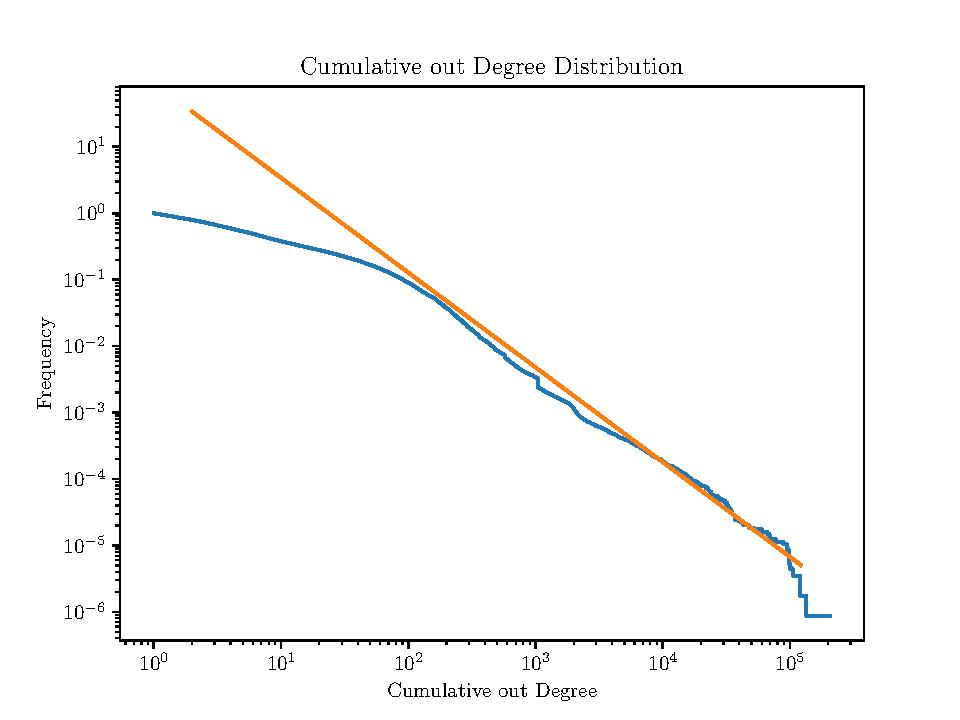
\includegraphics[width=\linewidth]{wikipedia_pt_in.pdf}
		\caption{Cumulative in-degree distribution.}
		\label{fig:inddist}
	\end{subfigure}
	\begin{subfigure}{.475\textwidth}
		\centering
		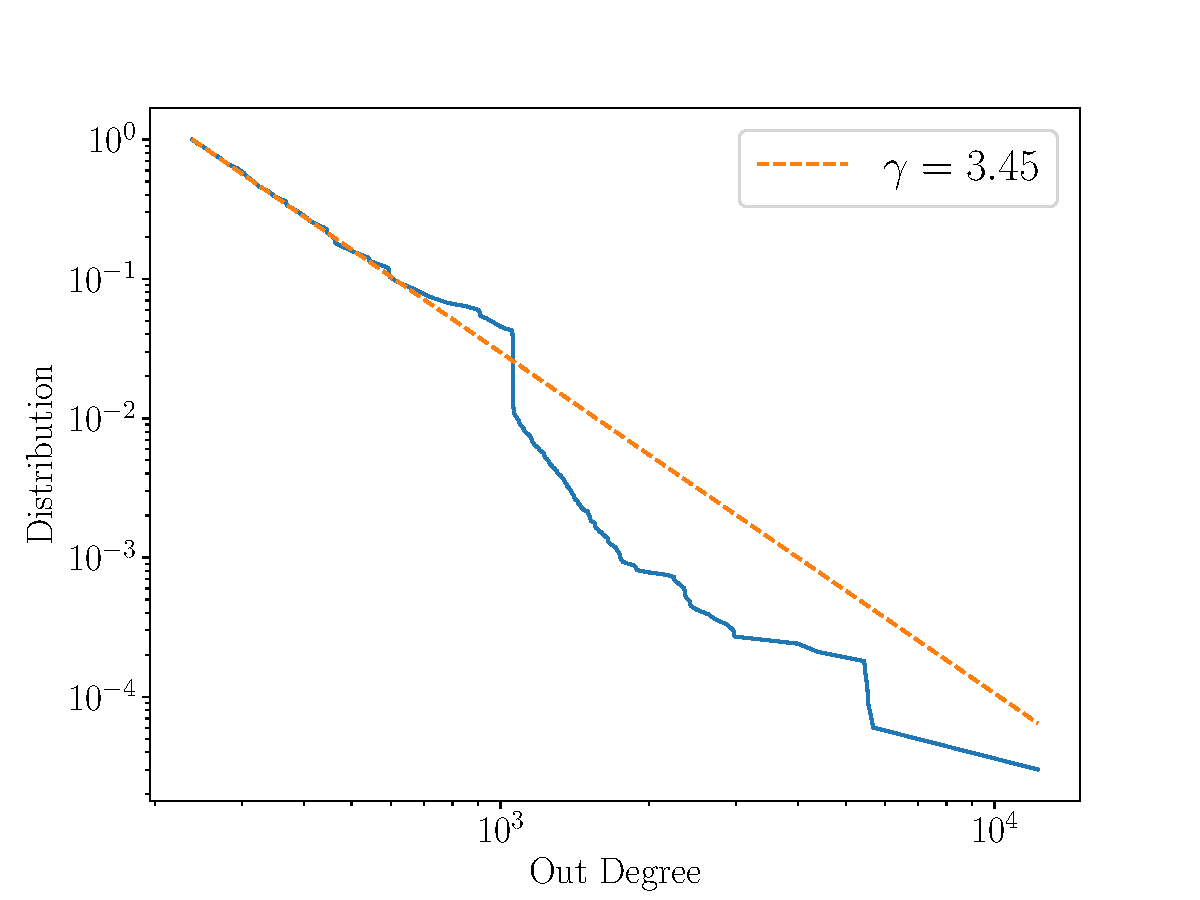
\includegraphics[width=\linewidth]{wikipedia_pt_out.pdf}
		\caption{Cumulative out-degree distribution.}
		\label{fig:outddist}
	\end{subfigure}
	\caption{Degree distributions.}
\end{figure}

In figures ~\ref{fig:inddist} and~\ref{fig:outddist} we present the cumulative in and out, respectively, degree distributions and their approximate power law regression. The regression was obtained using a simplified method based on the one described by Clauset et al. \cite{Clauset2009}.

\begin{figure}[h]
	\centering
	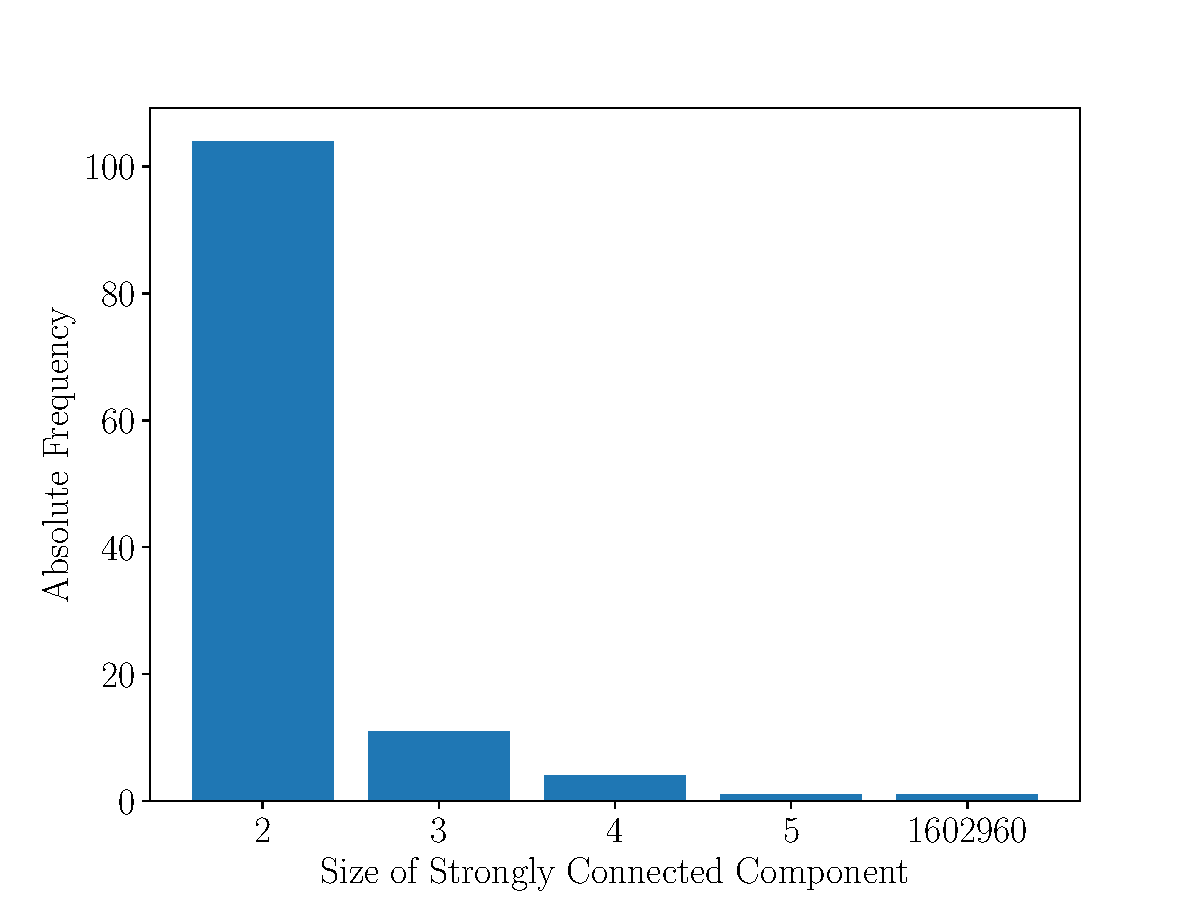
\includegraphics[width=\linewidth]{wikipedia_pt_sccdistr.pdf}
	\caption{Strongly Connected Component distribution.}
	\label{fig:sccdist}
\end{figure}

Figure \ref{fig:sccdist} shows the number of \acrshort{scc} with respect to their cardinality. We notice a giant strongly connected component, as would be expected.

\begin{figure}[h]
	\centering
	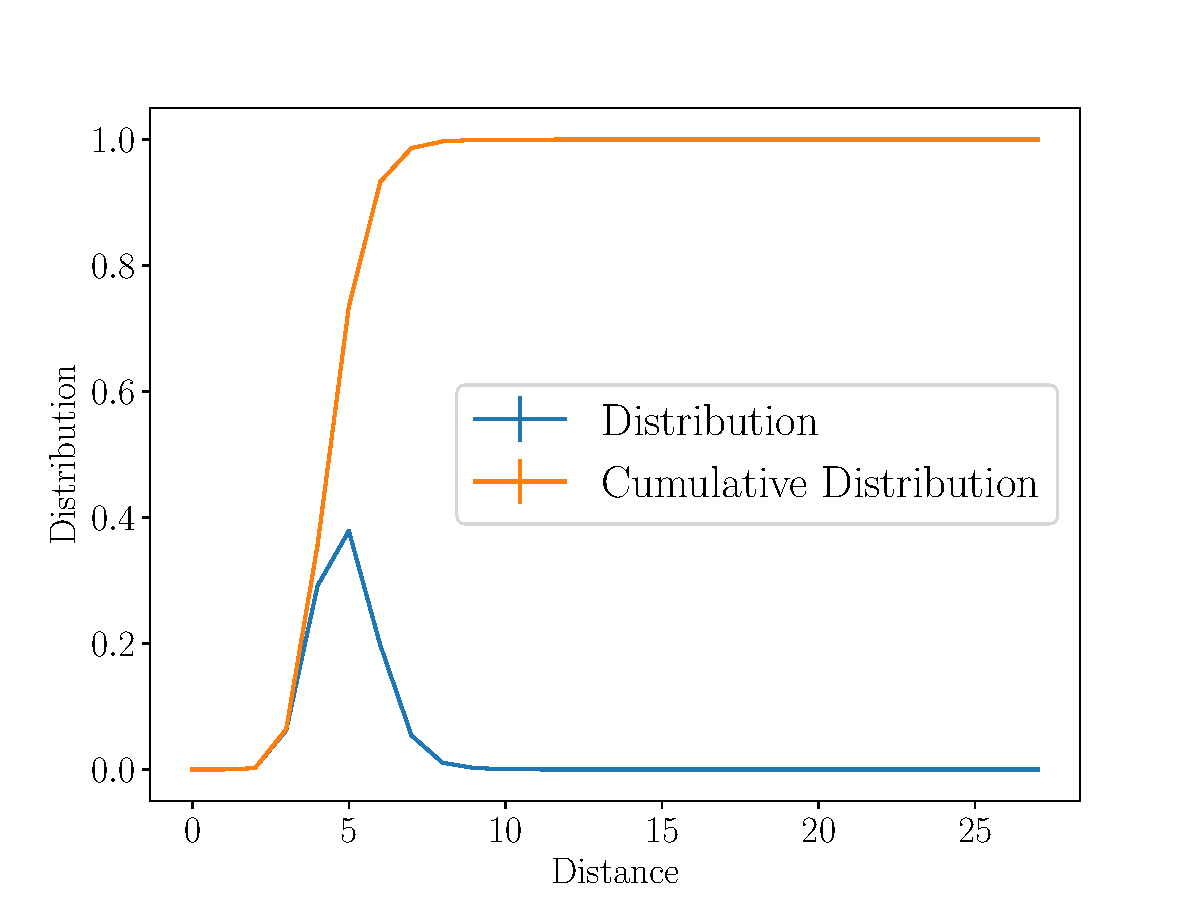
\includegraphics[width=\linewidth]{wikipedia_pt_neighbourhood_function.pdf}
	\caption{Approximate neighbourhood function.}
	\label{fig:neighfun}
\end{figure}

In figure \ref{fig:neighfun} is represented the approximate neighbourhood function as computed by Webgraph. This measure represents for each $t \in N$, the number of pairs of nodes $ \langle x, y \rangle $ such that $y$ is reachable from $x$ in less than $t$ hops \cite{Boldi2011HyperANFAT}.

We have also obtained an estimation of the average path length through HyperBall \cite{DBLP:conf/icdm/BoldiV13}. The estimated value is $ 4.9290 \pm 0.0026 $. This result reinforces what has been previously discussed, as it can be seen in Figure \ref{fig:neighfun} roughly a half of the nodes can be reached from each other in just 5 hops.

\begin{figure}[h]
	\centering
	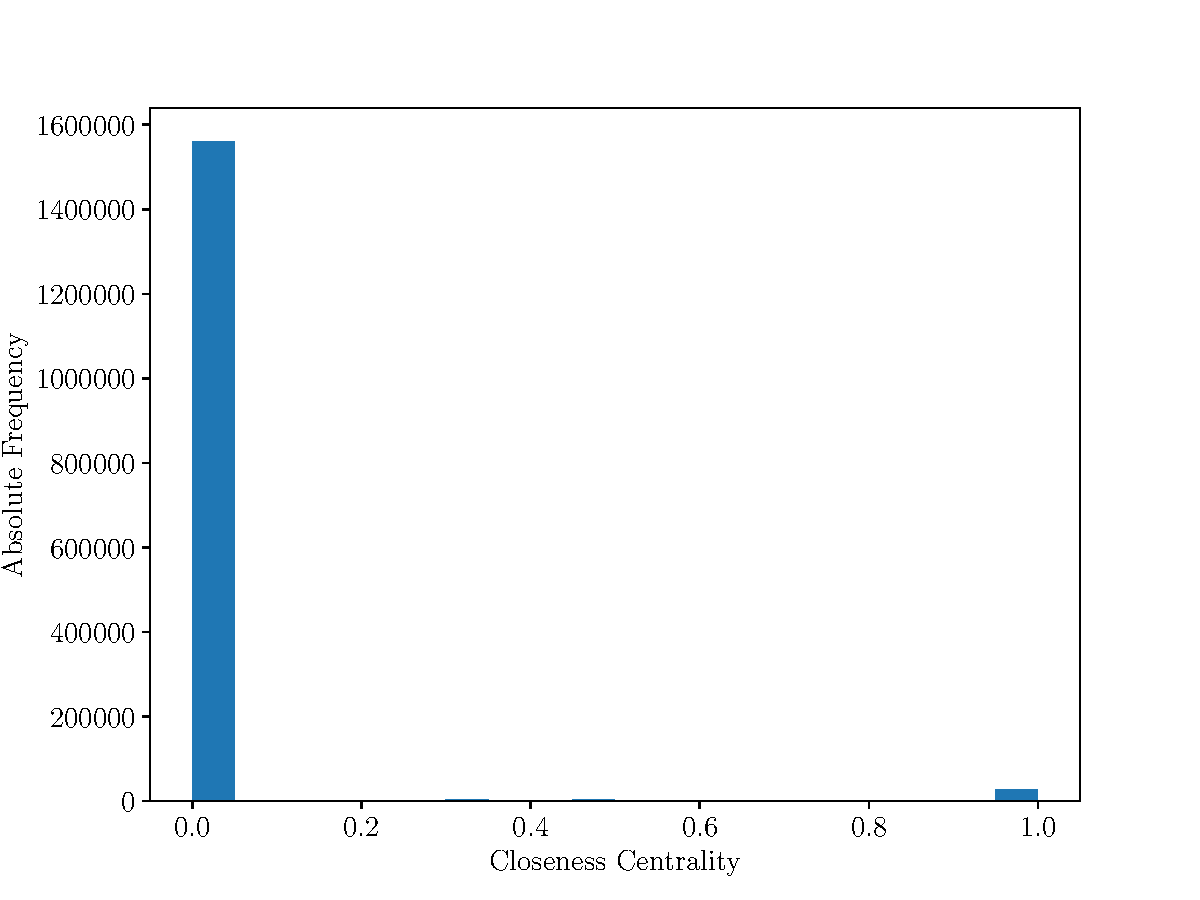
\includegraphics[width=\linewidth]{wikipedia_pt_closeness_centrality.pdf}
	\caption{Approximate neighbourhood function.}
	\label{fig:closeness}
\end{figure}

\begin{figure}[h]
	\centering
	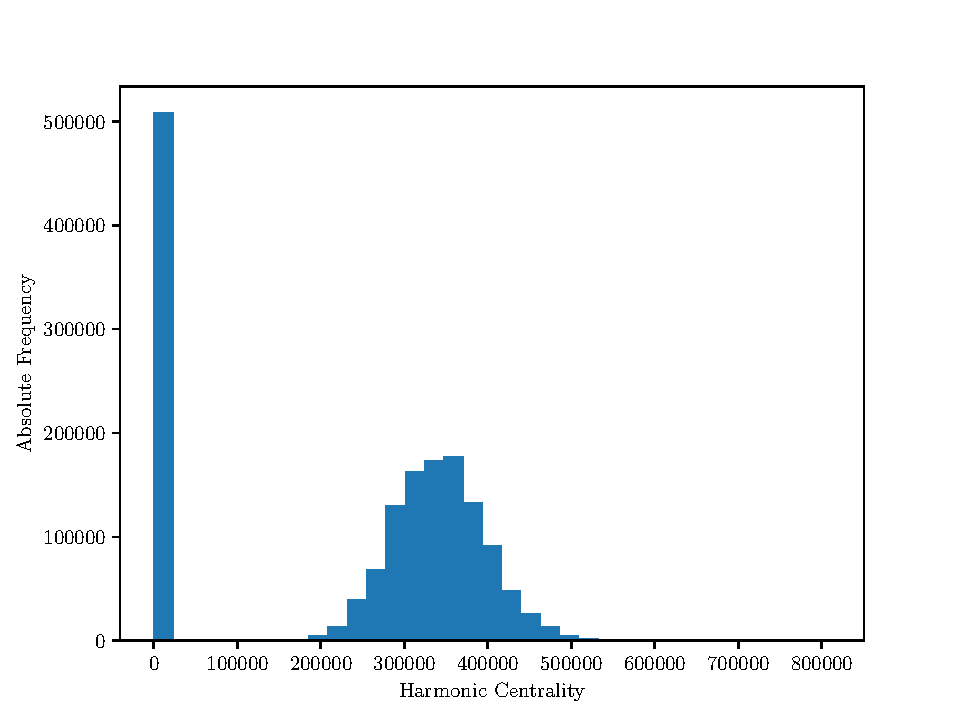
\includegraphics[width=\linewidth]{wikipedia_pt_harmonic_centrality.pdf}
	\caption{Approximate neighbourhood function.}
	\label{fig:harmonic}
\end{figure}

Out of curiosity we decided to estimate the closeness centrality, and the results are just as expected. As it can be seen in Figure~\ref{fig:closeness} almost all nodes have a closeness centrality of 0, this is due to our graph not being connected. Since this measure does not give us any further information on the graph, we also decided to calculate the harmonic centrality, which nicely allows the existence of disconnected nodes by giving them less weight than to the closer vertices, which means their contribution is close to 0. Figure~\ref{fig:harmonic} exhibits the obtained results.

\section{Discussion}

The cumulative in-degree $\gamma = 2.42$ parameter is lower than its out-degree counterpart $\gamma = 3.89$. Although our data is unlabelled, we believe this phenomenon occurs because there are few Wikipedia pages which reference most of the others (ie. indexes), leading to a higher $\gamma$ in the out-degree distribution. Conversely, the in-degree distribution parameter $\gamma = 2.42$ is lower because pages are comparatively more uniformly referenced.

In what regards the \acrshort{scc}s, as previously mentioned, we have found a giant one %ugly
containing almost all the nodes ($1\,602\,960$) in the graph, and also a very few small ones. These results are in accordance with the average degrees ($> ln(N)$) obtained, which imply a connected regime.

By analysing the approximate neighbourhood function, we have concluded that at around 10 hops, all the reachable nodes become connected.

Small world cenas ln n / ln k = 4.2 parecido. random graph


comparar resultado analitico com a estimativa scale


The variance for the in-degree distribution is 290301.58. This result is also expected, the power-law distribution has a $\gamma = 2.42$ implying a divergent variance for an infinite set. The variance of the out-degree distribution is significantly lower 5394.48, which is also expected, since the $ \gamma = 3.89 $ which implies a finite variance, hence the lower value.

Effective diameter is a more robust measure of the diameter, which calculates the diameter using 90\% as a cut-off of the cumulative probability function. We obtained an effective diameter of $5.8361 \pm 0.0022$.


SPID -> acima de um para redes reais, 

\printglossary[type=\acronymtype]

\bibliographystyle{plain}
\bibliography{references}

\end{document}
